\documentclass{controle}
\usepackage{main}

\title{Exercice : Fonction Exponentielle}
\author{Quentin Canu}
\date{Aujourd'hui}

\begin{document}
\maketitle

On étudie une fonction $f$ définie sur $[-2;5]$. Sa courbe représentative $\mathcal{C}_f$ est donnée sur le repère ci-dessous :
\begin{center}
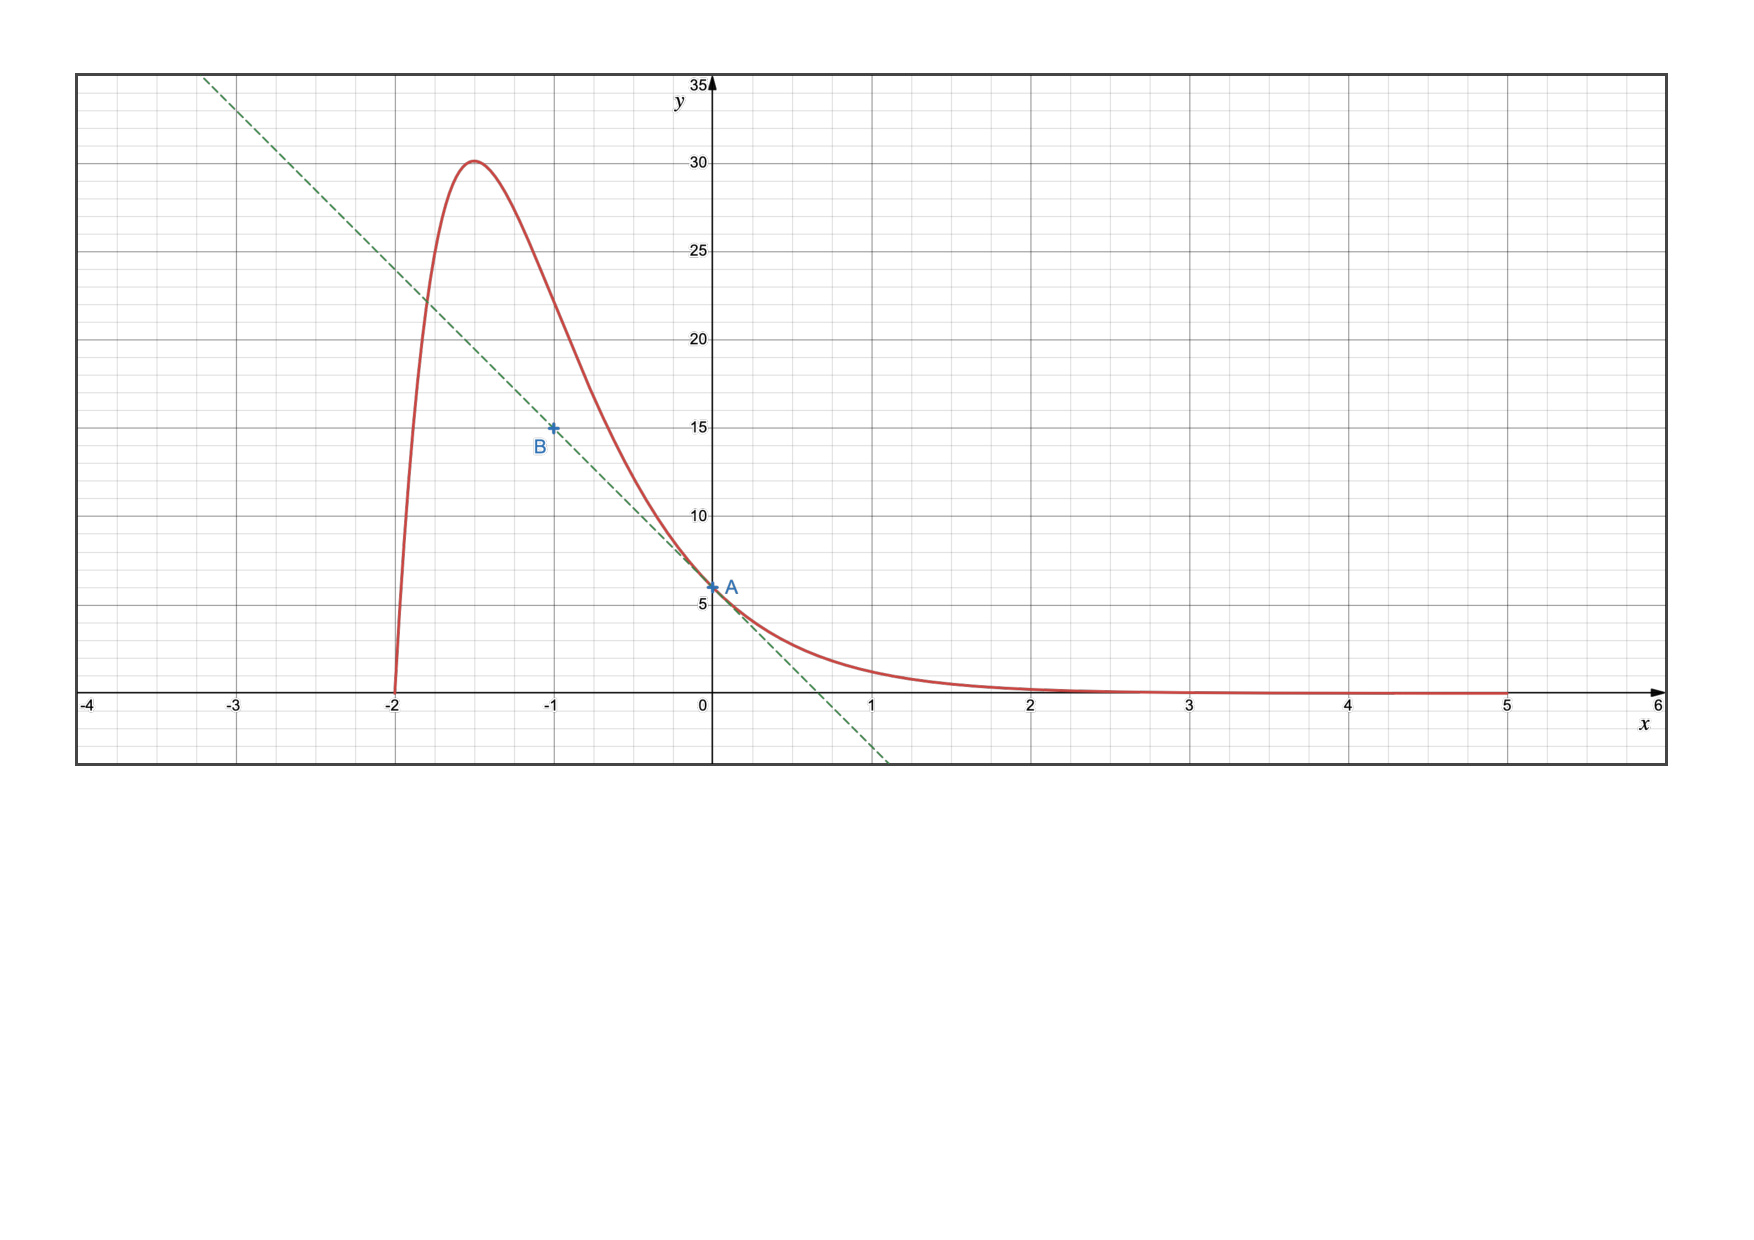
\includegraphics[width=\textwidth,trim={0 6cm 0 0}, clip]{Graphique_expo.pdf}
\end{center}
On admet que la fonction est dérivable sur $]-2;5[$.
\begin{parts}
\part[0.5] Déterminer graphiquement $f(0)$ et $f'(0)$.
\part[0.5] Résoudre graphiquement, à l'aide de la précision permise par le graphique, l'équation suivante :
\begin{equation*}
f'(x) = 0
\end{equation*}
\part[1] On admet que pour tout $x \in [-2;5]$, on a 
\begin{equation*}
f(x)=(3x+6)e^{-2x}
\end{equation*}
En déduire que $f'(x) = (-6x-9)e^{-2x}$ pour tout $x \in ]-2;5[$.
\part[1] Étudier le signe de $f'$. Justifier votre réponse.
\part[0.5] En déduire le tableau de variations de $f$.
\part[0.5] Soit $A(0;f(0))$. Donner l'équation de la tangente à $\mathcal{C}_f$ passant par $A$, nommée $d$.
\part[1] En déduire le point d'intersection de $d$ et de l'axe des abscisses.
\end{parts}
\end{document}